\documentclass{standalone}
\usepackage{tikz}
\usepackage{amsmath}
\usetikzlibrary{matrix}
\usetikzlibrary {shapes.geometric}
\begin{document}
    
        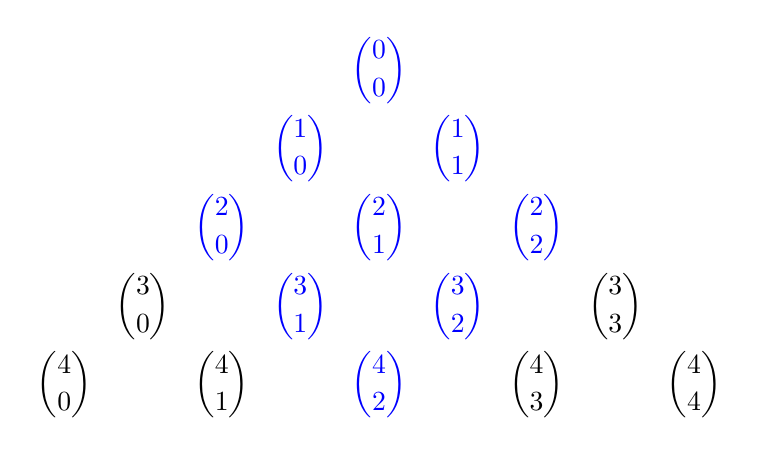
\begin{tikzpicture}

            %\draw [help lines] (0,0) grid (10,10); 

            \path   (5,10)  node (a) [] {\textcolor {blue}{\mbox{$\displaystyle \binom{0}{0}$ }}}
                    (4,9) node (b) [] {\textcolor {blue}{\mbox{$\displaystyle \binom{1}{0}$ }}}
                    (6,9) node (c) [] {\textcolor {blue}{\mbox{$\displaystyle \binom{1}{1}$ }}}
                    (3,8) node (d) [] {\textcolor {blue}{\mbox{$\displaystyle \binom{2}{0}$ }}}
                    (5,8) node (e) [] {\textcolor {blue}{\mbox{$\displaystyle \binom{2}{1}$ }}}
                    (7,8) node (f) [] {\textcolor {blue}{\mbox{$\displaystyle \binom{2}{2}$ }}}
                    (2,7) node (g) [] {\mbox{$\displaystyle \binom{3}{0}$ }}
                    (4,7) node (h) [] {\textcolor {blue}{\mbox{$\displaystyle \binom{3}{1}$ }}}
                    (6,7) node (i) [] {\textcolor {blue}{\mbox{$\displaystyle \binom{3}{2}$ }}}
                    (8,7) node (j) [] {\mbox{$\displaystyle \binom{3}{3}$ }}
                    (1,6) node (k) [] {\mbox{$\displaystyle \binom{4}{0}$ }}
                    (3,6) node (l) [] {\mbox{$\displaystyle \binom{4}{1}$ }}
                    (5,6) node (m) [] {\textcolor {blue}{\mbox{$\displaystyle \binom{4}{2}$ }}}
                    (7,6) node (n) [] {\mbox{$\displaystyle \binom{4}{3}$ }}
                    (9,6) node (o) [] {\mbox{$\displaystyle \binom{4}{4}$ }};
                
        \end{tikzpicture}

\end{document}